\scanpage{25}
% L1–3
Soient $\lambda=\sum_{b\in B}\lambda_b e_b$, $\mu=\sum_{b\in\unsure{B|D}}\mu_b e_b$ deux éléments de $C$
($\lambda_{-b}=-\lambda_b$, $|\lambda_b|\leq 1$, idem pour $\mu$) quand a-t-on
$R(\lambda,\mu)$ (relation d'équiv. des facettes ?)

% L4–10
Si $\lambda\ne\mu$, on veut que \deleted{\unsure{On}} $\exists\,t\in\mathbb R$, $t\lambda+(1-t)\mu\in C$,
avec au choix $t<0$, ou $t>1$. \deleted{\unsure{Pour le|Pour les}} On veut
\deleted{$t\lambda_b\unsure{+}$} donc $|t\lambda_b+(1-t)\mu_b|\leq1$. Si $\lambda_b=\mu_b$,
aucun Pb, si $|\lambda_b|,|\mu_b|<1$, non plus
le seul Pb si $\lambda_b\ne\mu_b$, et $\lambda_b\ \unsure{\underline{\text{ou}}|=}\ \mu_b=\pm1$
\figure{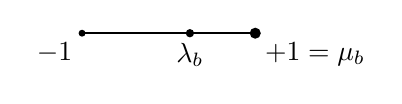
\begin{tikzpicture}[x=1cm,y=1cm]
\draw[thick](0,0)--(2.2,0);
\fill (0,0) circle (1.25pt) node[below left]{$-1$};
\fill (1.37,0) circle (1.5pt) node[below]{$\lambda_b$};
\fill (2.2,0) circle (2pt) node[below right]{$+1=\mu_b$};
\end{tikzpicture}}
Il faut donc
\[
\begin{aligned}
&|\lambda_b|=1\ \text{\uline{ou}}\ |\mu_b|=1\\
&\Longrightarrow\lambda_b=\mu_b\qquad\deleted{\unsure{\text{d}|\text{donc}}}
\end{aligned}
\]

% L11–14
Donc \deleted{a) L'ens \unsure{$J(\mu)$|$J(\lambda)$} des $\lambda$}

a) Soit $J(\lambda)=\{b\in B\mid\lambda_b\deleted{\unsure{\in}}=\pm1\}$. On veut $J(\lambda)=J(\mu)$ soit $J$

b) Si $j\in J$, on veut $\lambda_b=\mu_b$

La proposition s'ensuit.

% L15–18
\uline{Corollaire} La relation d'ordre entre facettes
de $C=C(B,R)$ est inverse de la relation de
prolongement entre sections partielles de
$B$ sur $I=B/R$.

% L19–24
La facette maximale correspond à la section
partielle vide ($J=\varnothing$). Les facettes sous-maximales correspondent aux éléments de $B$.
Deux facettes ss-maximales distinctes \inserted{\deleted{\unsure{se}} ne} se rencontrent
pas (``sont $//$'') ssi elles correspondent à des pts
$x,y$ de $B$ qui sont congrus par $R$.
% archive sheet number: 24
